% PREAMBLE
\documentclass[11pt]{amsart}
\usepackage[T1]{fontenc}
\usepackage{lmodern}
\usepackage{microtype}
\usepackage{amsmath,amssymb}
\usepackage{mathtools}
\usepackage{graphicx}
\usepackage{booktabs}
\usepackage{tikz}
\usepackage[colorlinks=true,linkcolor=blue!45!black,citecolor=blue!45!black,urlcolor=blue!45!black]{hyperref}
\usepackage[capitalize]{cleveref}

\newtheorem{theorem}{Theorem}[section]
\newtheorem{proposition}[theorem]{Proposition}
\newtheorem{lemma}[theorem]{Lemma}
\newtheorem{corollary}[theorem]{Corollary}
\newtheorem{conjecture}[theorem]{Conjecture}
\theoremstyle{definition}
\newtheorem{definition}[theorem]{Definition}
\newtheorem{fact}[theorem]{Fact}
\theoremstyle{remark}
\newtheorem{remark}[theorem]{Remark}

\title{Divisor Avatars: Which Parity Designs Count the Divisors of a Power}
\author{Carlo Mitchener}
\address{MrlyProd, Inc.}
\email{carlo.mitchener@gmail.com}
\date{First published 2026-08-23, revised 2026-09-02}

% PAPER
\begin{document}

\begin{abstract}
Colour the cells of a cube by whether their coordinates are odd or even, keep a chosen set of colours, and count what you kept. This paper shows that the resulting count is often the number of divisors of a power, and settles exactly when. For an integer $x$ with $\omega(x)=D$ distinct prime factors, a design of dimension $D$ whose cell count at side $2n+1$ equals $d(x^{n})$ for every $n \ge 0$ exists if and only if $\Omega(x) \le 2\omega(x)$; when it exists its weight signature is forced, and the number of such designs is a product of binomial coefficients. The qualifying divisor polynomials in dimension $D$ number $\sum_{m \le D} p(m)$, the partition sums A000070. The Menger sponge is the boundary case: its fill is $d(240^{n})$ and its void count is A395241.
\end{abstract}

\begin{center}

\includegraphics[width=0.36\textwidth]{figures/avatar.png}
\end{center}
\maketitle

\section{Introduction}
\label{sec:intro}

Take a cube of $3 \times 3 \times 3$ small cells and number the coordinates $1,2,3$. Throw away every cell that has at least two even coordinates. Seven cells go: the one in the very middle, and the six in the middles of the faces. Twenty stay. That is the first step of the Menger sponge, and it is drawn in \cref{fig:sponge}.

\begin{figure}[ht]
\centering
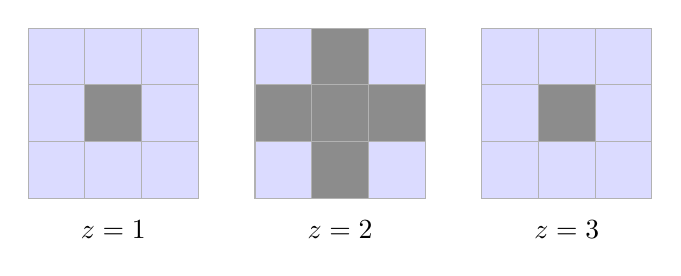
\begin{tikzpicture}[scale=0.72]
\begin{scope}[shift={(0,0)}]
\foreach \i in {1,2,3} \foreach \j in {1,2,3} {\fill[blue!14] (\i-1,\j-1) rectangle (\i,\j);}
\fill[black!45] (1,1) rectangle (2,2);
\draw[step=1,gray!60] (0,0) grid (3,3);
\draw[gray!60] (0,0) rectangle (3,3);
\node at (1.5,-0.55) {$z=1$};
\end{scope}
\begin{scope}[shift={(4,0)}]
\foreach \i in {1,2,3} \foreach \j in {1,2,3} {\fill[blue!14] (\i-1,\j-1) rectangle (\i,\j);}
\foreach \p in {{(1,0)},{(0,1)},{(1,1)},{(2,1)},{(1,2)}} {\fill[black!45] \p rectangle ++(1,1);}
\draw[step=1,gray!60] (0,0) grid (3,3);
\draw[gray!60] (0,0) rectangle (3,3);
\node at (1.5,-0.55) {$z=2$};
\end{scope}
\begin{scope}[shift={(8,0)}]
\foreach \i in {1,2,3} \foreach \j in {1,2,3} {\fill[blue!14] (\i-1,\j-1) rectangle (\i,\j);}
\fill[black!45] (1,1) rectangle (2,2);
\draw[step=1,gray!60] (0,0) grid (3,3);
\draw[gray!60] (0,0) rectangle (3,3);
\node at (1.5,-0.55) {$z=3$};
\end{scope}
\end{tikzpicture}
\caption{The first Menger step at side $3$, one layer at a time. Dark cells have at least two even coordinates and are removed; $7$ go and $20$ stay. Now $20 = d(240)$, and the coincidence is not one: at side $2n+1$ the same rule keeps exactly $d(240^{n})$ cells.}
\label{fig:sponge}
\end{figure}

Now enlarge the cube to side $5$, then $7$, then $2n+1$, applying the same rule. The counts are $1, 20, 81, 208, 425, \dots$. They are the divisor counts of the powers of $240$:
\[
  d(240^{n}) = (4n+1)(n+1)^{2}, \qquad d(240^{0})=1,\; d(240)=20,\; d(240^{2})=81 .
\]
So a purely geometric census -- how many cells survive an odd/even rule -- is computing an arithmetic function. That is the phenomenon this paper is about.

The rule is completely specified by which parity patterns it keeps. In dimension $D$ a \emph{design} is a set $F$ of parity patterns, a subset of $\{0,1\}^{D}$, and the design's \emph{fill} at side $2n+1$ is the number of cells whose parity pattern lies in $F$. The Menger rule is the design that keeps every pattern with at most one even coordinate. Call a design a \emph{divisor avatar} of $x$ when its fill equals $d(x^{n})$ at every $n \ge 0$.

Two questions follow immediately. Which integers $x$ have an avatar? And how many designs realise one? The answer to the first is a single clean inequality between the two standard prime-counting functions: $\Omega(x)$, the number of prime factors with multiplicity, and $\omega(x)$, the number of distinct ones.

\begin{quote}
\textbf{An integer $x>1$ has a divisor avatar if and only if $\Omega(x) \le 2\,\omega(x)$.}
\end{quote}

The Menger sponge sits exactly on the boundary: $240 = 2^{4}\cdot 3 \cdot 5$ has $\Omega = 6$ and $\omega = 3$. Push one prime factor further -- to $480$, with $\Omega = 7$ -- and no design in any dimension has that fill. The obstruction is not subtle once you see it: the fill of a $D$-dimensional design cannot count more than $\binom{D}{1}=D$ parity patterns of weight one, and the arithmetic demands $\sum_{i}(a_{i}-1)$ of them. When the inequality does hold the design is essentially forced: its weight signature is determined outright, and only the choice of which patterns to take at each weight is free, giving $\prod_{w}\binom{\binom{D}{w}}{f_{w}}$ designs. Counting the qualifying polynomials in dimension $D$ turns into counting partitions, and the answer is $\sum_{m \le D} p(m)$, the sequence A000070 \cite{a000070}: $2, 4, 7, 12, 19, 30, \dots$

\subsection*{What is and is not new here}

The fill of a design is an Ehrhart-type count: lattice points of a dilated box that lie in prescribed cosets of $(2\mathbb{Z})^{D}$, and such counts are quasi-polynomial by the standard theory \cite{beckrobins}. Restricted to odd sides they are honest polynomials, and \cref{lem:fill} is a two-line special case, not an application of the general machinery. The formula $d(x^{n}) = \prod_{i}(a_{i}n+1)$ is classical \cite{apostol}. The change of basis that turns one into the other -- substituting $a_{i}n+1 = (a_{i}-1)n + (n+1)$ -- is one line and no depth is claimed for it.

What is new is the pair of questions above and their answers: the realizability criterion $\Omega(x) \le 2\omega(x)$ (\cref{thm:criterion}), the count $\prod_{w}\binom{\binom{D}{w}}{f_{w}}$ of designs realizing it, the A000070 census (\cref{cor:census}), and the splitting test that decides an avatar from its fill polynomial alone (\cref{cor:split}). The closed form for the Menger void count is the author's own OEIS entry A395241 \cite{a395241}, whose name field already records $a(n)=n^{2}(4n+3)$ and whose comments already record the Menger reading and the anchor $a(1)=7$; \cref{prop:void} supplies that entry's missing derivation and is presented as such, not as a new result.

\Cref{sec:def} sets up designs and fills. \Cref{sec:res} states everything. \Cref{sec:proofs} proves it. A short arithmetic tour rides along: which divisor-sum functions can and cannot be counted by a polynomial (\cref{prop:sigmak}), what happens to Robin's inequality along the seven three-dimensional avatar ladders (\cref{prop:robin}), and a machine scan of every three-dimensional design against nine observables (\cref{fact:scan}).

\section{Definitions}
\label{sec:def}

Throughout, $D \ge 0$ is an integer, $p_{1} < p_{2} < \cdots$ are the primes, $d$ is the number-of-divisors function, $\sigma_{k}(m)=\sum_{e \mid m} e^{k}$ and $\sigma = \sigma_{1}$, $\omega(x)$ is the number of distinct primes dividing $x$ and $\Omega(x)$ the number counted with multiplicity. For a vector $b=(b_{1},\dots,b_{D})$, $e_{w}(b)$ is the $w$-th elementary symmetric polynomial, with $e_{0}(b)=1$ and $e_{w}(b)=0$ for $w>D$. Finally $p(m)$ is the number of partitions of $m$.

\begin{definition}[design]
\label{def:design}
The \emph{parity cube} in dimension $D$ is $\{0,1\}^{D}$; its elements are called \emph{corners}, and the \emph{weight} of a corner $c$ is $|c| = c_{1}+\cdots+c_{D}$. A \emph{design} is a subset $F \subseteq \{0,1\}^{D}$. Its \emph{weight signature} is the vector $f=(f_{0},\dots,f_{D})$ with
\[
  f_{w} = \#\{\,c \in F : |c| = w\,\}.
\]
In dimension $D=0$ the parity cube $\{0,1\}^{0}$ has a single element, the empty corner, of weight $0$; so dimension zero has exactly two designs, $\emptyset$ and $\{()\}$, of signatures $(0)$ and $(1)$.
\end{definition}

\begin{definition}[fill]
\label{def:fill}
Let $B_{n} = \{1,2,\dots,2n+1\}^{D}$ be the cubical grid of odd side $2n+1$, its cells addressed by integer coordinates. The \emph{parity} of a cell $u \in B_{n}$ is the corner $\pi(u) \in \{0,1\}^{D}$ with $\pi(u)_{i}=1$ when $u_{i}$ is even and $\pi(u)_{i}=0$ when $u_{i}$ is odd. A cell is \emph{filled} by $F$ when $\pi(u) \in F$, and the \emph{fill} of $F$ is
\[
  P_{F}(n) = \#\{\, u \in B_{n} : \pi(u) \in F \,\}, \qquad n \ge 0 .
\]
The \emph{void} of $F$ is $V_{F}(n) = (2n+1)^{D} - P_{F}(n)$.
\end{definition}

\begin{definition}[divisor avatar]
\label{def:avatar}
A design $F$ of dimension $D$ is a \emph{divisor avatar} of the integer $x > 1$ when
\[
  P_{F}(n) = d(x^{n}) \quad \text{for every integer } n \ge 0 .
\]
We then call $x$ an \emph{avatar integer} of $F$, and the least such $x$ the \emph{minimal avatar}.
\end{definition}

\begin{definition}[Menger design]
\label{def:menger}
The \emph{Menger design} is $F_{M} = \{\, c \in \{0,1\}^{3} : |c| \le 1 \,\}$, of signature $(1,3,0,0)$. Its filled cells are exactly those with at most one even coordinate, so its voids are exactly the cells removed by the first step of the Menger sponge construction at side $2n+1$.
\end{definition}

\begin{definition}[the touched complex]
\label{def:touched}
Realise each cell $u \in B_{n}$ as the closed unit box $\prod_{i}[u_{i}-1,u_{i}] \subset \mathbb{R}^{D}$. A vertex, edge or $2$-face of the unit grid of $\mathbb{R}^{D}$ is \emph{touched} by $F$ when it lies in the box of some cell filled by $F$; write $\mathrm{ver}_{F}(n)$, $\mathrm{edg}_{F}(n)$, $\mathrm{fac}_{F}(n)$ for the numbers of touched vertices, edges and $2$-faces. Two filled cells are \emph{adjacent} when their boxes share a $(D-1)$-face; let $\mathrm{adj}_{F}(n)$ count the adjacent pairs, $\kappa_{F}(n)$ the connected components of the filled cells under adjacency, and $\mathrm{sur}_{F}(n)$ the $(D-1)$-faces lying in exactly one filled box. The \emph{cycle rank} of $F$ is $\mathrm{adj}_{F}(n) - P_{F}(n) + \kappa_{F}(n)$, and in dimension three the \emph{Euler characteristic} of $F$ is
\[
  \chi_{F}(n) = \mathrm{ver}_{F}(n) - \mathrm{edg}_{F}(n) + \mathrm{fac}_{F}(n) - P_{F}(n).
\]
\end{definition}

\section{Results}
\label{sec:res}

\subsection*{The fill is a polynomial, and the polynomial remembers the design}

\begin{lemma}[fill law]
\label{lem:fill}
For every design $F$ of dimension $D$ and every $n \ge 0$,
\[
  P_{F}(n) = \sum_{w=0}^{D} f_{w}\,(n+1)^{D-w}\,n^{w} .
\]
In particular $P_{F}$ agrees on $n \ge 0$ with a polynomial of degree $D$ and leading coefficient $|F|$ when $F \neq \emptyset$, and with the zero polynomial otherwise.
\end{lemma}

\begin{lemma}[the fill basis is a basis]
\label{lem:basis}
The $D+1$ polynomials $q_{w}(n) = (n+1)^{D-w}n^{w}$, $w=0,\dots,D$, are linearly independent over $\mathbb{Q}$. Consequently the fill polynomial of a design determines its weight signature.
\end{lemma}

\begin{lemma}[realizability]
\label{lem:real}
A vector $f = (f_{0},\dots,f_{D})$ of integers is the weight signature of some design of dimension $D$ if and only if $0 \le f_{w} \le \binom{D}{w}$ for every $w$. The number of designs with that signature is $\prod_{w=0}^{D}\binom{\binom{D}{w}}{f_{w}}$.
\end{lemma}

\begin{lemma}[binomial domination]
\label{lem:dom}
Let $b_{1},\dots,b_{D}$ be nonnegative integers with $m = b_{1}+\cdots+b_{D}$. Then
\[
  0 \le e_{w}(b) \le \binom{m}{w} \qquad (0 \le w \le D),
\]
and hence $e_{w}(b) \le \binom{D}{w}$ for every $w$ whenever $m \le D$.
\end{lemma}

\subsection*{The criterion}

\begin{theorem}[avatar criterion]
\label{thm:criterion}
Let $x > 1$ be an integer with $x = q_{1}^{a_{1}}\cdots q_{D}^{a_{D}}$ over its $D = \omega(x)$ distinct prime divisors $q_{1} < \cdots < q_{D}$, every $a_{i} \ge 1$, and put $b_{i} = a_{i}-1$. Then:
\begin{enumerate}
\item[(i)] $\displaystyle d(x^{n}) = \sum_{w=0}^{D} e_{w}(b)\,(n+1)^{D-w}n^{w}$ for every $n \ge 0$, as an identity of polynomials in $n$;
\item[(ii)] a design $F$ of dimension $D$ satisfies $P_{F}(n)=d(x^{n})$ for every $n \ge 0$ if and only if its weight signature is $f_{w} = e_{w}(b)$ for every $w$;
\item[(iii)] such a design exists if and only if
\[
  \Omega(x) \;\le\; 2\,\omega(x), \qquad \text{equivalently} \qquad \sum_{i=1}^{D}(a_{i}-1) \le D ;
\]
\item[(iv)] when it exists, the number of such designs is exactly $\displaystyle \prod_{w=0}^{D}\binom{\binom{D}{w}}{e_{w}(b)}$;
\item[(v)] no design of any dimension other than $D$ has fill polynomial $d(x^{n})$.
\end{enumerate}
\end{theorem}

\begin{remark}
\label{rem:thedesign}
Part (iv) is the reason one must say ``any design with signature $e_{w}(b)$'' and never ``the design''. For $x=240$ the signature $(1,3,0,0)$ in dimension $3$ is realised by $\binom{1}{1}\binom{3}{3}\binom{3}{0}\binom{1}{0}=1$ design, so the Menger design is unique; but for $x = 2\cdot 3 \cdot 5$ the signature is $(1,0,0,0)$, realised by $\binom{1}{1}\binom{3}{0}\binom{3}{0}\binom{1}{0}=1$ design, while for $x = 2^{2}\cdot 3 \cdot 5$ the signature $(1,1,0,0)$ is realised by $\binom{3}{1}=3$ distinct designs, all with the same fill.
\end{remark}

\begin{remark}
\label{rem:sharp}
The failure is real and not rare. The smallest failing $x$ is $x=8$: $D=1$, $b=(2)$, and the demanded signature $(1,2)$ needs $f_{1}=2 > \binom{1}{1}=1$. In dimension two, $x=72=2^{3}3^{2}$ demands $(1,3,2)$ against the caps $(1,2,1)$; exhaustive search over all $16$ designs of dimension two confirms that $d(72^{n})=6n^{2}+5n+1$ is not among the $12$ distinct fill polynomials available there.
\end{remark}

\begin{corollary}[splitting criterion]
\label{cor:split}
Let $F$ be a nonempty design of dimension $D$. Then $F$ is a divisor avatar of some integer $x$ with $\omega(x)=D$ if and only if
\[
  P_{F}(0) = 1 \quad\text{and}\quad P_{F} \text{ splits into linear factors over } \mathbb{Q}.
\]
In that case $P_{F}(n) = \prod_{i=1}^{D}(a_{i}n+1)$ with every $a_{i}$ a positive integer, the avatar integers of $F$ are exactly the $\prod_{i} p_{\tau(i)}^{a_{i}}$ over injections $\tau$ into the primes, and the minimal avatar is obtained by pairing the largest slope with the smallest prime.
\end{corollary}

\begin{corollary}[census of qualifying polynomials]
\label{cor:census}
For every $D \ge 0$ the number of distinct polynomials of the form $d(x^{n})$ with $\omega(x)=D$ that arise as the fill of some design of dimension $D$ equals
\[
  \sum_{m=0}^{D} p(m) = \mathrm{A000070}(D).
\]
For $D = 0,1,2,\dots,8$ these are $1, 2, 4, 7, 12, 19, 30, 45, 67$.
\end{corollary}

\subsection*{The Menger sponge, both halves}

\begin{proposition}[void census]
\label{prop:void}
In the cubical grid of side $2n+1$, the number of cells having at least two even coordinates is
\[
  a(n) = 3n^{2}(n+1) + n^{3} = n^{2}(4n+3),
\]
with $a(1)=7$: the central cell and the six face centres. This is the closed form recorded in A395241 \cite{a395241}; the proposition supplies its derivation.
\end{proposition}

\begin{corollary}[the sponge is a boundary avatar]
\label{cor:bridge}
The Menger design $F_{M}$ of \cref{def:menger} has
\begin{gather*}
  P_{F_{M}}(n) = (n+1)^{2}(4n+1) = 4n^{3}+9n^{2}+6n+1 = d(240^{n}),\\
  V_{F_{M}}(n) = (2n+1)^{3} - P_{F_{M}}(n) = n^{2}(4n+3),
\end{gather*}
so its fill is a divisor avatar with minimal avatar $240$ and its void is A395241. Moreover $\Omega(240)=6=2\,\omega(240)$, so $240$ lies exactly on the boundary of \cref{thm:criterion}(iii), while $480$, with $\Omega=7$ and $\omega=3$, has no avatar in any dimension.
\end{corollary}

\begin{remark}
\label{rem:bridge}
\Cref{cor:bridge} is the complement identity $P+V=(2n+1)^{3}$ with both halves already on record: the fill polynomial follows from \cref{lem:fill} by expansion, and the void is A395241 \cite{a395241}. It is offered as the paper's worked example, not as a discovery.
\end{remark}

\subsection*{Which divisor functions a polynomial can count}

\begin{proposition}[divisor sums are excluded]
\label{prop:sigmak}
Let $Q$ be a polynomial in $n$ with rational coefficients. Then:
\begin{enumerate}
\item[(i)] $Q(n) = \sigma_{k}(x^{n})$ for every $n \ge 0$ is impossible for every integer $k \ge 1$ and every $x > 1$;
\item[(ii)] $Q(n) = \sigma(x^{n})/x^{n}$ for every $n \ge 0$ is impossible for every $x > 1$.
\end{enumerate}
At $x = 1$ both expressions collapse to the constant $1 = d(1^{n})$. Since every fill is a polynomial (\cref{lem:fill}), no design in any dimension has fill $\sigma_{k}(x^{n})$ or $\sigma(x^{n})/x^{n}$ for any $x > 1$: among the functions $\sigma_{k}$ only $k=0$, the divisor count itself, is ever the fill of a design.
\end{proposition}

\subsection*{The seven three-dimensional ladders and Robin's inequality}

Exactly seven integers occur as minimal avatars of three-dimensional designs, namely $30, 60, 120, 180, 240, 360, 900$; they are $5$-smooth because a minimal avatar in dimension three puts its exponents on the primes $2,3,5$, which is forced by minimality and is not an arithmetic accident. Robin's theorem \cite{robin} states that the Riemann Hypothesis is equivalent to $\sigma(N) < e^{\gamma}N\log\log N$ for all $N > 5040$.

\begin{proposition}[the corridors recede, for all $n$]
\label{prop:robin}
Let $x>1$ have prime support $\{2,3,5\}$, which covers all seven ladders. Then for every $n \ge 1$
\[
  1 < \frac{\sigma(x^{n})}{x^{n}} < \frac{15}{4},
  \qquad
  \lim_{n \to \infty}\frac{\sigma(x^{n})}{x^{n}} = \frac{15}{4},
  \qquad
  \lim_{n \to \infty}\frac{\sigma(x^{n})}{x^{n}\log\log(x^{n})} = 0 .
\]
Consequently $\sigma(N) < e^{\gamma}N\log\log N$ holds for every such power $N = x^{n}$ with
\[
  \log\log N > \frac{15}{4e^{\gamma}} = 2.10547306\ldots,
  \qquad \text{that is} \qquad N > 3681.171813\ldots,
\]
and in particular for every one of them exceeding $5040$. No computation is needed for any of this.
\end{proposition}

\begin{fact}[the corridor table]
\label{fact:robin}
Over the exact finite domain consisting of the $140$ powers $N = x^{n}$ with $x \in \{30,60,120,180,240,360,900\}$ and $1 \le n \le 20$, exactly $131$ of the powers satisfy $N > 5040$, and every one of those $131$ satisfies Robin's inequality. The domain is $140$ powers but only $130$ distinct integers, since $900^{n} = 30^{2n}$; the $131$ powers above $5040$ are $122$ distinct integers. The largest ratio $\sigma(N)/(N\log\log N)$ among them occurs at $N = 14400 = 120^{2}$ and equals $1.573259905933$ to twelve decimal places, against $e^{\gamma} = 1.781072417990$. Checked by \texttt{scripts/verify.py} with exact integer $\sigma$ and $40$-digit decimal arithmetic.
\end{fact}

\begin{remark}
\label{rem:norh}
\Cref{fact:robin} is illustration, not evidence: \cref{prop:robin} already proves the inequality on all seven ladders for all $n$, with no computation. And neither bears on the Riemann Hypothesis. Robin's criterion quantifies over all $N > 5040$; it suffices to check the colossally abundant numbers \cite{robin}, and the least counterexample, should one exist, must be superabundant \cite{akbaryfriggstad}. Verifying the inequality on a sparse family of powers excludes nothing. Identities describe; only a bound over the full domain constrains.
\end{remark}

\subsection*{Colossally abundant numbers}

\begin{fact}[the first colossally abundant number with no avatar]
\label{fact:ca}
Over the exact finite domain consisting of the first $13$ colossally abundant numbers A004490 \cite{a004490}, namely
\begin{gather*}
  2,\; 6,\; 12,\; 60,\; 120,\; 360,\; 2520,\; 5040,\\
  55440,\; 720720,\; 1441440,\; 4324320,\; 21621600,
\end{gather*}
the first twelve satisfy $\Omega \le 2\omega$ and therefore have divisor avatars by \cref{thm:criterion}, while the thirteenth,
\[
  21621600 = 2^{5}\cdot 3^{3}\cdot 5^{2}\cdot 7 \cdot 11 \cdot 13, \qquad \Omega = 13, \quad \omega = 6,
\]
has $\Omega = 13 > 12 = 2\omega$ and therefore has no avatar: no design, in any dimension, has fill $d(21621600^{n})$. Checked by \texttt{scripts/verify.py}.
\end{fact}

\begin{remark}
\label{rem:ca}
\Cref{fact:ca} corrects a natural guess. Colossally abundant numbers have exactly the shape $p_{1}^{a_{1}}p_{2}^{a_{2}}\cdots p_{D}^{a_{D}}$ with $a_{1} \ge \cdots \ge a_{D} \ge 1$ \cite{alaogluerdos}, which is the minimal-avatar shape, and this makes it tempting to claim that every colossally abundant number is a minimal avatar in dimension $\omega$. That claim is false, and $21621600$ refutes it. The correct statement is the criterion: a colossally abundant number has an avatar exactly when $\Omega \le 2\omega$. Surjectivity fails too, and badly: dimension $D$ carries $\mathrm{A000070}(D)$ qualifying polynomials against a handful of colossally abundant numbers.
\end{remark}

\subsection*{A machine scan in dimension three}

The group generated by coordinate permutations and coordinate reversals has order $48$ and acts on the $256$ designs of dimension three with $22$ orbits. Coding a design as $\sum_{c \in F}2^{c_{1}+2c_{2}+4c_{3}}$, take the least code in each orbit as its representative. Note that a coordinate reversal moves the odd/even origin, so it does \emph{not} preserve the fill at a fixed odd side; the scan below therefore classifies the $22$ canonical least-mask representatives, not all $256$ oriented masks.

Before the scan, one general fact about the observables of \cref{def:touched}. The fill is a disjoint union of boxes, which is why \cref{lem:fill} is a one-line count. The touched counts are unions of boxes that overlap, so they need inclusion-exclusion; the point of the next lemma is that the overlaps stay inside a small family of intervals whose sizes are linear in $n$.

\begin{lemma}[box unions are polynomial]
\label{lem:boxes}
For $n \ge 0$ set
\begin{gather*}
  O = \{1,3,\dots,2n+1\},\qquad E = \{2,4,\dots,2n\},\\
  O^{+} = \{0,1,\dots,2n+1\},\qquad E^{+} = \{1,2,\dots,2n\},
\end{gather*}
and let $\mathcal{S}_{n} = \{\,\emptyset,\; O \cap E^{+},\; O,\; E,\; E^{+},\; O^{+}\,\}$, of cardinalities $0,\,n,\,n+1,\,n,\,2n,\,2n+2$. Then $\mathcal{S}_{n}$ is closed under intersection, and if $B_{1},\dots,B_{r}$ are boxes $B_{k} = \prod_{i=1}^{D}U_{k,i}$ with every $U_{k,i} \in \mathcal{S}_{n}$ chosen by a rule independent of $n$, then $|B_{1} \cup \cdots \cup B_{r}|$ agrees for all $n \ge 0$ with a polynomial in $n$ of degree at most $D$.
\end{lemma}

\begin{proposition}[the local counts are polynomial]
\label{prop:topo}
Let $F$ be a design of dimension $D$. Then each of $\mathrm{ver}_{F}$, $\mathrm{edg}_{F}$, $\mathrm{fac}_{F}$, $\mathrm{sur}_{F}$ and $\mathrm{adj}_{F}$ agrees for all $n \ge 0$ with a polynomial in $n$ of degree at most $D$. Consequently, in dimension three the Euler characteristic $\chi_{F}$ agrees for all $n \ge 0$ with a polynomial of degree at most three; and in any dimension the cycle rank agrees with a polynomial on a given set of sides exactly when the component count $\kappa_{F}$ does, since the two differ by $\mathrm{adj}_{F}-P_{F}$.
\end{proposition}

\begin{fact}[extended avatar scan]
\label{fact:scan}
Over the exact finite domain consisting of the $22$ least-mask orbit representatives of dimension three, the nine observables
\begin{gather*}
  \text{fill},\quad \text{voids},\quad \text{surface},\quad \text{touched vertices},\quad \text{touched edges},\\
  \text{touched faces},\quad \text{Euler characteristic},\quad \text{components},\quad \text{cycle rank},
\end{gather*}
and the eleven sides $2n+1$ for $n=0,1,\dots,10$ (largest grid $21^{3} = 9261$ cells, every count literal, no sampling), the following hold. Every one of the $198$ observable sequences agrees on that range with a polynomial of degree at most three except the component and cycle-rank sequences of codes $30$ and $126$, which do so only for $n \ge 1$. Among the sequences that are of the form $d(x^{n})$ for all $n$ in range with $x>1$, exactly eight are not fills:
\begin{center}
\begin{tabular}{rlll}
\toprule
code & design & observable & law \\
\midrule
$0$  & $\emptyset$ & voids & $(2n+1)^{3} = d(900^{n})$\\
$1$  & $\{000\}$ & Euler characteristic & $(n+1)^{3} = d(30^{n})$\\
$1$  & $\{000\}$ & components & $(n+1)^{3} = d(30^{n})$\\
$3$  & $\{000,100\}$ & Euler characteristic & $(n+1)^{2} = d(6^{n})$\\
$3$  & $\{000,100\}$ & components & $(n+1)^{2} = d(6^{n})$\\
$7$  & $\{000,100,010\}$ & components & $n+1 = d(2^{n})$\\
$15$ & $\{000,100,010,110\}$ & Euler characteristic & $n+1 = d(2^{n})$\\
$15$ & $\{000,100,010,110\}$ & components & $n+1 = d(2^{n})$\\
\bottomrule
\end{tabular}
\end{center}
There are in addition exactly nine sequences that are constantly $1 = d(1^{n})$: components for the codes $23, 27, 31, 61, 63, 111, 127, 255$ and Euler characteristic for code $255$. Finally, exactly eight representatives have a fill of the form $d(x^{n})$ with $x>1$, namely codes $1,3,7,15,23,27,63,255$ with minimal avatars $30,60,120,180,240,180,360,900$. Checked by \texttt{scripts/verify.py}, which recomputes all nine observables cell by cell, recovers each law by exact rational interpolation, and applies \cref{cor:split}.
\end{fact}

\begin{conjecture}[the component count is polynomial in every dimension]
\label{con:topo}
For every design $F$ in every dimension $D$ there is a polynomial that agrees with the component count $\kappa_{F}(n)$ for all sufficiently large $n$. \emph{Evidence:} \cref{fact:scan} exhibits such a polynomial for all $22$ orbit representatives in dimension three over $n = 0,\dots,10$, of degree at most three in every case, agreeing from $n=0$ for twenty of them and from $n=1$ for the two exceptions, codes $30$ and $126$. By \cref{prop:topo} the same statement for the cycle rank is equivalent to this one; the corresponding statements for the touched counts and for the Euler characteristic are not conjectural but proved, and hold from $n=0$. \emph{Failure modes:} the component count is the one observable here that is not a union-of-boxes census, so \cref{lem:boxes} does not reach it; two filled regions can merge into one component only at sides above a threshold, and nothing in the present argument bounds that threshold. The count could be quasi-polynomial with a nontrivial period, or eventually polynomial with more exceptional small sides than the two seen in dimension three, and nothing here bounds the number of exceptional sides in dimension $D \ge 4$.
\end{conjecture}

\section{Proofs}
\label{sec:proofs}

\begin{proof}[Proof of \cref{lem:fill}]
Among $1,2,\dots,2n+1$ there are exactly $n+1$ odd values and exactly $n$ even values. Fix a corner $c \in \{0,1\}^{D}$. A cell $x \in B_{n}$ has $\pi(x)=c$ precisely when, for each coordinate $i$ independently, $x_{i}$ is even if $c_{i}=1$ and odd if $c_{i}=0$. The choices in distinct coordinates are independent, so the number of cells with $\pi(x)=c$ is $n^{|c|}(n+1)^{D-|c|}$. Summing over $c \in F$ and grouping the corners of equal weight gives the stated formula. Each term $q_{w}(n)=(n+1)^{D-w}n^{w}$ is a monic polynomial of degree $D$, so $P_{F}$ is a polynomial of degree at most $D$ whose coefficient of $n^{D}$ is $\sum_{w}f_{w}=|F|$; this is nonzero exactly when $F \neq \emptyset$.
\end{proof}

\begin{proof}[Proof of \cref{lem:basis}]
Suppose $\sum_{w=0}^{D}\lambda_{w}q_{w} = 0$ with $\lambda_{w} \in \mathbb{Q}$. We show $\lambda_{0}=\cdots=\lambda_{D}=0$ by induction on $w$. Evaluating at $n=0$ kills every term with $w \ge 1$ and leaves $\lambda_{0}(0+1)^{D}=\lambda_{0}$, so $\lambda_{0}=0$. Assume $\lambda_{0}=\cdots=\lambda_{j-1}=0$ for some $j \ge 1$. Then $\sum_{w \ge j}\lambda_{w}(n+1)^{D-w}n^{w}=0$ identically, and every term is divisible by $n^{j}$ in $\mathbb{Q}[n]$; dividing by $n^{j}$ gives $\sum_{w \ge j}\lambda_{w}(n+1)^{D-w}n^{w-j}=0$ identically. Evaluating at $n=0$ now kills every term with $w>j$ and leaves $\lambda_{j}=0$. This completes the induction. Since $P_{F}=\sum_{w}f_{w}q_{w}$ by \cref{lem:fill}, and a polynomial identity holding for all $n \ge 0$ holds identically, the coefficients $f_{w}$ are determined by $P_{F}$.
\end{proof}

\begin{proof}[Proof of \cref{lem:real}]
There are exactly $\binom{D}{w}$ corners of weight $w$, so any signature must satisfy $0 \le f_{w} \le \binom{D}{w}$. Conversely, given such a vector, choose any $f_{w}$ of the weight-$w$ corners for each $w$ and take $F$ to be the union; the choices at distinct weights are independent, so this both realises $f$ and counts the designs realising it as $\prod_{w}\binom{\binom{D}{w}}{f_{w}}$.
\end{proof}

\begin{proof}[Proof of \cref{lem:dom}]
For $A = \sum_{w}A_{w}t^{w}$ and $B=\sum_{w}B_{w}t^{w}$, say that $A$ is dominated by $B$, written $A \preceq B$, when $0 \le A_{w} \le B_{w}$ for every $w$. Domination is preserved by products of polynomials with nonnegative coefficients: if $A \preceq A'$ and $B \preceq B'$ then the coefficient of $t^{w}$ in $AB$ is $\sum_{j}A_{j}B_{w-j} \le \sum_{j}A'_{j}B'_{w-j}$, the coefficient of $t^{w}$ in $A'B'$.

For a nonnegative integer $b$ we have $1+bt \preceq (1+t)^{b}$, since the coefficients on the left are $1, b, 0, 0, \dots$ and those on the right are $1, b, \binom{b}{2}, \dots$, all nonnegative. Multiplying these $D$ dominations together,
\[
  \sum_{w}e_{w}(b)\,t^{w} \;=\; \prod_{i=1}^{D}(1+b_{i}t) \;\preceq\; \prod_{i=1}^{D}(1+t)^{b_{i}} \;=\; (1+t)^{m},
\]
which is exactly $0 \le e_{w}(b) \le \binom{m}{w}$ for every $w$. If moreover $m \le D$ then $\binom{m}{w} \le \binom{D}{w}$ for every $w \ge 0$, since $\binom{m}{w}$ is nondecreasing in $m$.
\end{proof}

\begin{proof}[Proof of \cref{thm:criterion}]
(i) Since $x^{n} = \prod_{i}q_{i}^{a_{i}n}$ with the $q_{i}$ distinct, $d(x^{n}) = \prod_{i=1}^{D}(a_{i}n+1)$. Write $b_{i}=a_{i}-1 \ge 0$. Then
\[
  a_{i}n+1 = (a_{i}-1)n + (n+1) = b_{i}n + (n+1),
\]
so, expanding the product by choosing from each factor either the term $b_{i}n$ or the term $(n+1)$,
\begin{align*}
  \prod_{i=1}^{D}(a_{i}n+1)
  &= \prod_{i=1}^{D}\bigl(b_{i}n+(n+1)\bigr)\\
  &= \sum_{S \subseteq \{1,\dots,D\}} \Bigl(\prod_{i \in S}b_{i}\Bigr) n^{|S|}(n+1)^{D-|S|}\\
  &= \sum_{w=0}^{D} e_{w}(b)\,n^{w}(n+1)^{D-w},
\end{align*}
the last step grouping the subsets by their size. This is an identity in $\mathbb{Z}[n]$. (It is the generating-function identity $\prod_{i}(b_{i}t+1)=\sum_{w}e_{w}(b)t^{w}$ evaluated at $t=n/(n+1)$ and multiplied by $(n+1)^{D}$; the expansion above avoids the division and is valid at $n=-1$ as well.)

(ii) By \cref{lem:fill}, $P_{F} = \sum_{w}f_{w}q_{w}$; by (i), $d(x^{n}) = \sum_{w}e_{w}(b)q_{w}(n)$. Two polynomials agreeing at all integers $n \ge 0$ are equal, so $P_{F}(n)=d(x^{n})$ for all $n \ge 0$ is equivalent to $\sum_{w}\bigl(f_{w}-e_{w}(b)\bigr)q_{w}=0$, and by \cref{lem:basis} that forces $f_{w}=e_{w}(b)$ for every $w$. The converse is immediate from the same two displays.

(iii) By (ii) and \cref{lem:real}, a design with fill $d(x^{n})$ exists if and only if $0 \le e_{w}(b) \le \binom{D}{w}$ for every $w$. Necessity: taking $w=1$ gives $e_{1}(b)=\sum_{i}(a_{i}-1)=\Omega(x)-\omega(x) \le \binom{D}{1}=D=\omega(x)$, that is $\Omega(x) \le 2\omega(x)$. Sufficiency: if $\sum_{i}b_{i}=m \le D$ then \cref{lem:dom} gives $0 \le e_{w}(b) \le \binom{D}{w}$ for every $w$, so the signature is realizable.

(iv) Immediate from (ii) and the counting half of \cref{lem:real}.

(v) A design $F'$ of dimension $D' \ge 0$ has fill either identically zero (when $F'=\emptyset$) or a polynomial of degree exactly $D'$, by \cref{lem:fill}. The polynomial $d(x^{n}) = \prod_{i=1}^{D}(a_{i}n+1)$ has degree exactly $D$ and is not identically zero, so $D'=D$.
\end{proof}

\begin{proof}[Proof of \cref{cor:split}]
Suppose first that $F$ is a divisor avatar of $x$ with $\omega(x)=D$. Then $P_{F}(n)=\prod_{i}(a_{i}n+1)$ with each $a_{i} \ge 1$ an integer, which both splits over $\mathbb{Q}$ and gives $P_{F}(0)=1$.

Conversely, suppose $P_{F}(0)=1$ and $P_{F}$ splits into linear factors over $\mathbb{Q}$. Since $F \neq \emptyset$, \cref{lem:fill} gives $\deg P_{F}=D$ and $P_{F} \in \mathbb{Z}[n]$ with constant term $P_{F}(0)=f_{0}=1$. Write $P_{F}(n)=\sum_{j=0}^{D}c_{j}n^{j}$ with $c_{0}=1$, $c_{D}=|F| > 0$, and let
\[
  P^{*}_{F}(n) \;=\; n^{D}P_{F}(1/n) \;=\; \sum_{j=0}^{D}c_{j}n^{D-j} \;=\; n^{D} + c_{1}n^{D-1} + \cdots + c_{D},
\]
a \emph{monic} polynomial with integer coefficients. Because $P_{F}(0)=1 \neq 0$, no root of $P_{F}$ is zero, and the roots of $P^{*}_{F}$ are exactly the reciprocals of the roots of $P_{F}$. By hypothesis all $D$ roots of $P_{F}$ are rational, hence so are all $D$ roots of $P^{*}_{F}$; and by the rational root theorem every rational root of a monic integer polynomial is an integer. So the roots of $P_{F}$ are $-1/a_{1},\dots,-1/a_{D}$ for nonzero integers $a_{1},\dots,a_{D}$ (the sign is a labelling choice).

Each $a_{i}$ is positive. Indeed, by \cref{lem:fill}, $P_{F}(t)=\sum_{w}f_{w}(t+1)^{D-w}t^{w}$ has nonnegative coefficients $f_{w}$ not all zero, so for real $t>0$ every term is nonnegative and at least one is strictly positive, giving $P_{F}(t)>0$; and $P_{F}(0)=1>0$. Hence $P_{F}$ has no root in $[0,\infty)$, so every root $-1/a_{i}$ is negative, so every $a_{i}$ is positive.

Finally, $n+1/a_{i} = (a_{i}n+1)/a_{i}$, so $P_{F}(n) = \lambda\prod_{i}(a_{i}n+1)$ for some rational $\lambda$, and setting $n=0$ gives $\lambda = P_{F}(0)=1$. Thus $P_{F}(n)=\prod_{i}(a_{i}n+1)$, and for any injection $\tau$ from $\{1,\dots,D\}$ into the primes, $x = \prod_{i}p_{\tau(i)}^{a_{i}}$ satisfies $\omega(x)=D$ and $d(x^{n})=\prod_{i}(a_{i}n+1)=P_{F}(n)$.

Every avatar integer has that shape. Indeed, let $y>1$ be any avatar integer of $F$ and write $y = r_{1}^{c_{1}}\cdots r_{D'}^{c_{D'}}$ over its distinct primes with every $c_{i} \ge 1$. Then $\prod_{i}(c_{i}n+1) = d(y^{n}) = P_{F}(n) = \prod_{i}(a_{i}n+1)$ as polynomials, and a polynomial determines its multiset of roots, so $D'=D$ and $\{c_{1},\dots,c_{D}\} = \{a_{1},\dots,a_{D}\}$ as multisets. Hence the avatar integers of $F$ are exactly the $\prod_{i}p_{\tau(i)}^{a_{i}}$.

It remains to minimise over $\tau$. If some $\tau$ uses a prime $p_{k}$ while a smaller prime $p_{j}$, $j<k$, is unused, then replacing the factor $p_{k}^{a}$ by $p_{j}^{a}$ gives another avatar integer, with the same exponent multiset, that is strictly smaller because $a \ge 1$ and $p_{j} < p_{k}$. So a minimiser uses exactly the primes $p_{1},\dots,p_{D}$, and minimising $x$ is minimising $\prod_{i}p_{i}^{a_{\rho(i)}}$ over orderings $\rho$, which by the rearrangement inequality applied to $\sum_{i}a_{\rho(i)}\log p_{i}$ is achieved by pairing the largest exponent with the smallest prime.
\end{proof}

\begin{proof}[Proof of \cref{cor:census}]
By \cref{thm:criterion}, the polynomials in question are exactly the $\prod_{i=1}^{D}(a_{i}n+1)$ for multisets $\{a_{1},\dots,a_{D}\}$ of positive integers with $\sum_{i}(a_{i}-1) \le D$, and distinct multisets give distinct polynomials because a polynomial determines its multiset of roots. Substituting $b_{i}=a_{i}-1$, these are exactly the multisets of $D$ nonnegative integers with $\sum_{i}b_{i} \le D$. Dropping the zero entries, such a multiset is a partition of some integer $m$ with $0 \le m \le D$ into at most $D$ positive parts; and since every part is at least $1$, a partition of $m \le D$ automatically has at most $D$ parts. So the count is $\sum_{m=0}^{D}p(m)$, which is A000070$(D)$ \cite{a000070}. For $D=0,\dots,8$ the partial sums of $p(m)=1,1,2,3,5,7,11,15,22$ are $1,2,4,7,12,19,30,45,67$.
\end{proof}

\begin{proof}[Proof of \cref{prop:void}]
Number the coordinates from $1$ to $2n+1$; there are $n$ even values and $n+1$ odd values. A removed cell has either exactly two even coordinates or exactly three, and the two cases are disjoint. For exactly two: choose which two of the three coordinates are even, in $\binom{3}{2}=3$ ways; each even coordinate then has $n$ possible values and the remaining odd coordinate has $n+1$, giving $3n^{2}(n+1)$. For exactly three: $n^{3}$. Hence
\[
  a(n) = 3n^{2}(n+1) + n^{3} = 3n^{3}+3n^{2}+n^{3} = 4n^{3}+3n^{2} = n^{2}(4n+3).
\]
At $n=1$ this is $7$, namely the central cell $(2,2,2)$ and the six face centres $(2,2,1),(2,2,3),(2,1,2),(2,3,2),(1,2,2),(3,2,2)$.
\end{proof}

\begin{proof}[Proof of \cref{cor:bridge}]
The Menger design has signature $(1,3,0,0)$, so the fill law of \cref{lem:fill} gives
\[
  P_{F_{M}}(n) = (n+1)^{3} + 3(n+1)^{2}n = (n+1)^{2}\bigl((n+1)+3n\bigr) = (n+1)^{2}(4n+1).
\]
Since $240 = 2^{4}\cdot 3\cdot 5$ we have $d(240^{n}) = (4n+1)(n+1)(n+1)$, which is the same polynomial; equivalently $b=(3,0,0)$ and $e_{w}(b)=(1,3,0,0)$, matching \cref{thm:criterion}(ii). Subtracting from $(2n+1)^{3}=8n^{3}+12n^{2}+6n+1$ gives $V_{F_{M}}(n)=4n^{3}+3n^{2}=n^{2}(4n+3)$, which is \cref{prop:void} and A395241, as it must be since the cells $F_{M}$ discards are exactly those with at least two even coordinates. Finally $\Omega(240)=4+1+1=6$ and $\omega(240)=3$, so $\Omega=2\omega$; whereas $480=2^{5}\cdot 3\cdot 5$ has $\Omega=7>6=2\omega$, so by \cref{thm:criterion}(iii) and (v) no design in any dimension has fill $d(480^{n})$.
\end{proof}

\begin{proof}[Proof of \cref{prop:sigmak}]
(i) For $k \ge 1$ and $x > 1$ we have $\sigma_{k}(x^{n}) \ge x^{kn} \ge 2^{n}$, since $x^{n}$ is itself a divisor of $x^{n}$ and $x^{k} \ge 2$. A polynomial in $n$ of degree $\delta$ grows like $n^{\delta}$, while $2^{n}/n^{\delta} \to \infty$. So the two cannot agree for all large $n$, hence not for all $n \ge 0$.

(ii) Write $x = \prod_{p^{e}\|x}p^{e}$. Then
\[
  \frac{\sigma(x^{n})}{x^{n}} = \prod_{p^{e}\|x}\bigl(1+p^{-1}+\cdots+p^{-en}\bigr).
\]
This is a finite product of factors, each at least $1$ and each strictly increasing in $n$ (the factor for $p$ gains the positive term $p^{-en-1}+\cdots+p^{-en-e}$ when $n$ increases by one), so the product is strictly increasing in $n$. It is bounded above by $\prod_{p \mid x}(1-1/p)^{-1}$, a finite constant. A polynomial that is bounded on the nonnegative integers must be constant, since a nonconstant polynomial is unbounded there; but a strictly increasing sequence is not constant. Contradiction.

At $x=1$, $\sigma_{k}(1)=1$ and $\sigma(1)/1=1$ for every $n$, so both expressions are the constant $1=d(1^{n})$.
\end{proof}

\begin{proof}[Proof of \cref{prop:robin}]
Write $x = 2^{\alpha}3^{\beta}5^{\gamma}$ with $\alpha,\beta,\gamma \ge 1$; each of $30,\allowbreak 60,\allowbreak 120,\allowbreak 180,\allowbreak 240,\allowbreak 360,\allowbreak 900$ has this form. Then
\[
  \frac{\sigma(x^{n})}{x^{n}} = \prod_{p \in \{2,3,5\}}\bigl(1+p^{-1}+\cdots+p^{-e_{p}n}\bigr),
  \qquad (e_{2},e_{3},e_{5}) = (\alpha,\beta,\gamma).
\]
Each factor is a truncation of a convergent geometric series, so it is strictly less than $(1-1/p)^{-1}$ and increases to it as $n \to \infty$. Hence the product is strictly less than $2 \cdot \tfrac{3}{2}\cdot\tfrac{5}{4} = \tfrac{15}{4}$ and tends to $\tfrac{15}{4}$; it exceeds $1$ because every factor does. Since $\log\log(x^{n}) = \log(n\log x) \to \infty$, the third limit follows from the boundedness of the first ratio.

For the threshold: for $N = x^{n}$,
\[
  \frac{\sigma(N)}{N\log\log N} < \frac{15/4}{\log\log N},
\]
and the right side is less than $e^{\gamma}$ exactly when $\log\log N > \dfrac{15}{4e^{\gamma}}$. Numerically $e^{\gamma}=1.781072417990\ldots$, so $15/(4e^{\gamma}) = 2.105473063376\ldots$ and $\exp\exp\bigl(15/(4e^{\gamma})\bigr) = 3681.171813\ldots$. Every such power exceeding $3682$ therefore satisfies Robin's inequality, and in particular every one exceeding $5040$.
\end{proof}

\begin{proof}[Proof of \cref{lem:boxes}]
Write $O^{-} = O \cap E^{+} = \{1,3,\dots,2n-1\}$. Among the six members of $\mathcal{S}_{n}$ one has the inclusions $O^{-} \subseteq O \subseteq O^{+}$, $O^{-} \subseteq E^{+} \subseteq O^{+}$ and $E \subseteq E^{+}$, so every pair related by inclusion intersects inside the family. The pairs not so related are $(O,E)$ and $(O^{-},E)$, which meet in $\emptyset$ because one member consists of odd and the other of even integers, and $(O,E^{+})$, which meets in $O^{-}$ by definition. So $\mathcal{S}_{n}$ is closed under pairwise intersection, hence, being finite, under arbitrary intersections. Note that this table records which member the intersection is, and it is the same table for every $n \ge 0$.

Now let $B_{k} = \prod_{i}U_{k,i}$ be as stated. Intersections of boxes are computed slotwise, $\bigcap_{k \in G}B_{k} = \prod_{i}\bigl(\bigcap_{k \in G}U_{k,i}\bigr)$, so by the previous paragraph every such intersection is again a box all of whose slots carry members of $\mathcal{S}_{n}$, with the member in each slot named by a label that does not depend on $n$. Its cardinality is the product of the $D$ slot cardinalities, each one of $0, n, n+1, n, 2n, 2n+2$, hence a polynomial in $n$ of degree at most $D$. By inclusion-exclusion,
\[
  |B_{1} \cup \cdots \cup B_{r}| = \sum_{\emptyset \neq G \subseteq \{1,\dots,r\}}(-1)^{|G|+1}\Bigl|\bigcap_{k \in G}B_{k}\Bigr| ,
\]
a fixed integer combination, the same for every $n$, of polynomials of degree at most $D$.
\end{proof}

\begin{proof}[Proof of \cref{prop:topo}]
Write $T_{0}=O$, $T_{1}=E$, $T^{+}_{0}=O^{+}$, $T^{+}_{1}=E^{+}$, all members of $\mathcal{S}_{n}$. As in the proof of \cref{lem:fill}, the cells of $B_{n}$ of parity $c$ are exactly the box $\prod_{i}T_{c_{i}}$, and these boxes are pairwise disjoint over distinct corners $c$.

\emph{Vertices.} The vertices of the box of a cell $u$ are the points $v$ with $v_{i} \in \{u_{i}-1,u_{i}\}$ for every $i$. For a single slot, $\bigcup_{u_{i} \in O}\{u_{i}-1,u_{i}\} = O^{+}$ and $\bigcup_{u_{i} \in E}\{u_{i}-1,u_{i}\} = E^{+}$, and conversely each $v_{i} \in T^{+}_{c_{i}}$ is realised by some $u_{i} \in T_{c_{i}}$: if $v_{i}$ has the parity demanded by $c_{i}$ take $u_{i}=v_{i}$, otherwise take $u_{i}=v_{i}+1$, which stays in range in both cases. The slots are independent, so the vertices touched by the cells of parity $c$ are exactly the box $\prod_{i}T^{+}_{c_{i}}$, and $\mathrm{ver}_{F}(n) = \bigl|\bigcup_{c \in F}\prod_{i}T^{+}_{c_{i}}\bigr|$. Apply \cref{lem:boxes}.

\emph{Edges and $2$-faces.} An edge of the unit grid in direction $j$ is addressed by a cell coordinate in slot $j$ and a vertex coordinate in every other slot; the direction-$j$ edges of the box of $u$ are those with slot-$j$ value $u_{j}$ and slot-$i$ value in $\{u_{i}-1,u_{i}\}$ for $i \neq j$. By the same slotwise argument the direction-$j$ edges touched by the cells of parity $c$ form the box carrying $T_{c_{j}}$ in slot $j$ and $T^{+}_{c_{i}}$ elsewhere, so their union over $c \in F$ is covered by \cref{lem:boxes}; summing over the $D$ directions gives $\mathrm{edg}_{F}$. A $2$-face spanning slots $j$ and $k$ is addressed by cell coordinates in those two slots and vertex coordinates elsewhere, so the same argument with $T_{c_{j}},T_{c_{k}}$ in slots $j,k$ and $T^{+}_{c_{i}}$ elsewhere, summed over the $\binom{D}{2}$ pairs, gives $\mathrm{fac}_{F}$. Likewise a $(D-1)$-face omitting slot $j$ is addressed by a vertex coordinate in slot $j$ and cell coordinates elsewhere, giving $T^{+}_{c_{j}}$ in slot $j$ and $T_{c_{i}}$ elsewhere; call the resulting total $\Phi_{F}(n)$, again a polynomial of degree at most $D$. In dimension three $\Phi_{F}=\mathrm{fac}_{F}$, a $2$-face and a $(D-1)$-face being the same object there.

\emph{Adjacent pairs and surface.} Two cells are adjacent exactly when they differ by $e_{j}$ in a single slot $j$, and $\pi(u+e_{j})$ is $\pi(u)$ with slot $j$ flipped. So the lower cells of the direction-$j$ adjacent pairs of filled cells are those $u$ with $\pi(u)=c$ for some $c \in F$ with $c \oplus e_{j} \in F$, and $u_{j} \le 2n$: for each such $c$ this is the box carrying $T_{c_{j}} \cap E^{+}$ in slot $j$ and $T_{c_{i}}$ elsewhere, with $O \cap E^{+}$ and $E \cap E^{+} = E$ both in $\mathcal{S}_{n}$, and these boxes are disjoint over distinct $c$. Summing over $j$ and applying \cref{lem:boxes} makes $\mathrm{adj}_{F}$ a polynomial of degree at most $D$. Finally, a $(D-1)$-face omitting slot $j$, at vertex coordinate $v_{j}$, lies in the boxes of exactly those filled cells $u$ with the given coordinates elsewhere and $u_{j} \in \{v_{j},v_{j}+1\}$, so it lies in at most two filled boxes and in two precisely when that pair is adjacent. Hence $\Phi_{F} = \mathrm{sur}_{F} + \mathrm{adj}_{F}$ and $\mathrm{sur}_{F} = \Phi_{F} - \mathrm{adj}_{F}$ is a polynomial of degree at most $D$.

\emph{Euler characteristic and cycle rank.} In dimension three $\chi_{F} = \mathrm{ver}_{F} - \mathrm{edg}_{F} + \mathrm{fac}_{F} - P_{F}$, and $P_{F}$ is a polynomial of degree at most three by \cref{lem:fill}, so $\chi_{F}$ agrees with such a polynomial at every $n \ge 0$. In any dimension the cycle rank is $\mathrm{adj}_{F}-P_{F}+\kappa_{F}$, and $\mathrm{adj}_{F}-P_{F}$ is a polynomial, so on any set of sides the cycle rank agrees with a polynomial if and only if $\kappa_{F}$ does.
\end{proof}

\section{Reproducibility}
\label{sec:repro}

One script, \texttt{scripts/verify.py}, checks every number in this paper. It is plain \texttt{python3} with no dependencies beyond the standard library, takes no arguments, reads no files, and is run from the lane root as \texttt{python3 scripts/verify.py}. Total runtime is under two seconds on a laptop. Every assertion names both the value obtained and the value wanted, and the script exits nonzero on the first disagreement; a clean run prints one line per domain point and the word \texttt{all green}.

\begin{itemize}
\item \emph{Fill law} (\cref{lem:fill}). All $256$ designs of dimension three, all sides $2n+1$ for $n=0,\dots,6$: the cell-by-cell count is compared with $\sum_{w}f_{w}(n+1)^{3-w}n^{w}$.
\item \emph{Criterion} (\cref{thm:criterion}). Every integer $x$ with $2 \le x \le 3000$: the script factors $x$, tests $\Omega(x) \le 2\omega(x)$, and independently searches all $2^{2^{D}}$ designs of dimension $D=\omega(x)$ for one whose cell-by-cell fill matches $d(x^{n})$ at $n=0,\dots,6$, for $D \le 3$. The two verdicts must agree for every $x$ in range, and where a design exists the count of designs found must equal $\prod_{w}\binom{\binom{D}{w}}{e_{w}(b)}$.
\item \emph{Counterexamples} (\cref{rem:sharp}). $x=8$ in dimension one and $x=72$ in dimension two: the script enumerates the $4$ and $16$ designs respectively and asserts that $d(x^{n})$ is absent from the fill polynomials, reporting the $12$ distinct fill polynomials of dimension two.
\item \emph{Census} (\cref{cor:census}). Dimensions $D=0,\dots,8$: the number of distinct qualifying polynomials is enumerated directly from multisets and asserted equal to $\sum_{m \le D}p(m)$, giving $1,2,4,7,12,19,30,45,67$.
\item \emph{Sponge and void} (\cref{prop:void}, \cref{cor:bridge}). Sides $2n+1$ for $n=0,\dots,10$: the removed cells are counted literally and compared with $n^{2}(4n+3)$, the kept cells with $d(240^{n})$, and their sum with $(2n+1)^{3}$.
\item \emph{Robin corridors} (\cref{fact:robin}). The $140$ powers $x^{n}$ with $x \in \{30,\allowbreak 60,\allowbreak 120,\allowbreak 180,\allowbreak 240,\allowbreak 360,\allowbreak 900\}$ and $1 \le n \le 20$: $\sigma$ is computed exactly as an integer from the factorisation, the ratio in $40$-digit decimal arithmetic. The script asserts that the $140$ powers are $130$ distinct integers, that $131$ of the $140$ exceed $5040$ and are $122$ distinct integers, that all $131$ satisfy Robin's inequality, and that the maximum ratio is attained at $N=14400$ with value $1.573259905933$ to twelve places. It also checks the threshold constant $\exp\exp(15/(4e^{\gamma})) = 3681.17\ldots < 5040$.
\item \emph{Colossally abundant} (\cref{fact:ca}). The first $13$ terms of A004490: the criterion $\Omega \le 2\omega$ holds for the first twelve and fails at $21621600$.
\item \emph{Extended scan} (\cref{fact:scan}). The $22$ least-mask orbit representatives of dimension three, nine observables, $n=0,\dots,10$: every observable is recomputed cell by cell from the grid (components by union-find on face adjacency, cycle rank as graph edges minus fill plus components, Euler characteristic as touched vertices minus touched edges plus touched faces minus fill), each law is recovered by exact rational Lagrange interpolation and asserted to be a polynomial of degree at most three over the full range or over $n \ge 1$, and the splitting test of \cref{cor:split} is applied to every one of the $198$ sequences, the four late-starting ones included, over the full range $n=0,\dots,10$. The script asserts exactly the eight non-fill rows, exactly the nine constant identities, and exactly the eight fill avatars with their minimal avatars.
\end{itemize}

The figure in the lane README is regenerated by \texttt{scripts/figure.py}, also plain \texttt{python3}, run as \texttt{python3 scripts/figure.py}. It takes no input and writes \texttt{figures/sponge.svg} in well under a second.

\section*{Acknowledgments}

This paper was developed and verified in collaboration with Claude (Anthropic). The author takes sole responsibility for every claim.

\begin{thebibliography}{9}

\bibitem{akbaryfriggstad}
A. Akbary and Z. Friggstad, \emph{Superabundant numbers and the Riemann hypothesis}, Amer. Math. Monthly \textbf{116} (2009), no.~3, 273--275. \url{https://doi.org/10.4169/193009709X470128}

\bibitem{alaogluerdos}
L. Alaoglu and P. Erd\H{o}s, \emph{On highly composite and similar numbers}, Trans. Amer. Math. Soc. \textbf{56} (1944), 448--469. \url{https://doi.org/10.1090/S0002-9947-1944-0011087-2}

\bibitem{apostol}
T. M. Apostol, \emph{Introduction to Analytic Number Theory}, Springer, 1976. \url{https://doi.org/10.1007/978-1-4757-5579-4}

\bibitem{beckrobins}
M. Beck and S. Robins, \emph{Computing the Continuous Discretely: Integer-Point Enumeration in Polyhedra}, 2nd ed., Springer, 2015. \url{https://doi.org/10.1007/978-1-4939-2969-6}

\bibitem{robin}
G. Robin, \emph{Grandes valeurs de la fonction somme des diviseurs et hypoth\`ese de Riemann}, J. Math. Pures Appl. (9) \textbf{63} (1984), 187--213. \url{https://zbmath.org/0516.10036}

\bibitem{a000070}
OEIS Foundation Inc., \emph{Sequence A000070: partial sums of the partition numbers}, The On-Line Encyclopedia of Integer Sequences. \href{https://oeis.org/A000070}{https://oeis.org/A000070}

\bibitem{a004490}
OEIS Foundation Inc., \emph{Sequence A004490: colossally abundant numbers}, The On-Line Encyclopedia of Integer Sequences. \href{https://oeis.org/A004490}{https://oeis.org/A004490}

\bibitem{a395241}
C. Mitchener, \emph{Sequence A395241: $a(n) = n^{2}(4n+3)$}, The On-Line Encyclopedia of Integer Sequences, 2026. \href{https://oeis.org/A395241}{https://oeis.org/A395241}

\end{thebibliography}

\end{document}
